\documentclass[journal]{vgtc}                % final (journal style)
%\documentclass[review,journal]{vgtc}         % review (journal style)
%\documentclass[widereview]{vgtc}             % wide-spaced review
%\documentclass[preprint,journal]{vgtc}       % preprint (journal style)
%\documentclass[electronic,journal]{vgtc}     % electronic version, journal

%% Uncomment one of the lines above depending on where your paper is
%% in the conference process. ``review'' and ``widereview'' are for review
%% submission, ``preprint'' is for pre-publication, and the final version
%% doesn't use a specific qualifier. Further, ``electronic'' includes
%% hyperreferences for more convenient online viewing.

%% Please use one of the ``review'' options in combination with the
%% assigned online id (see below) ONLY if your paper uses a double blind
%% review process. Some conferences, like IEEE Vis and InfoVis, have NOT
%% in the past.

%% Please note that the use of figures other than the optional teaser is not permitted on the first page
%% of the journal version.  Figures should begin on the second page and be
%% in CMYK or Grey scale format, otherwise, colour shifting may occur
%% during the printing process.  Papers submitted with figures other than the optional teaser on the
%% first page will be refused.

%% These three lines bring in essential packages: ``mathptmx'' for Type 1
%% typefaces, ``graphicx'' for inclusion of EPS figures. and ``times''
%% for proper handling of the times font family.

\usepackage{mathptmx}
\usepackage{graphicx}
\usepackage{times}
\usepackage{balance}
\usepackage[nooneline,hang,it,IT]{subfigure}



%% We encourage the use of mathptmx for consistent usage of times font
%% throughout the proceedings. However, if you encounter conflicts
%% with other math-related packages, you may want to disable it.

%% This turns references into clickable hyperlinks.
\usepackage[bookmarks,backref=true,linkcolor=black]{hyperref} %,colorlinks
\hypersetup{
  pdfauthor = {},
  pdftitle = {},
  pdfsubject = {},
  pdfkeywords = {},
  colorlinks=true,
  linkcolor= black,
  citecolor= black,
  pageanchor=true,
  urlcolor = black,
  plainpages = false,
  linktocpage
}

%% If you are submitting a paper to a conference for review with a double
%% blind reviewing process, please replace the value ``0'' below with your
%% OnlineID. Otherwise, you may safely leave it at ``0''.
\onlineid{0}

%% declare the category of your paper, only shown in review mode
\vgtccategory{Research}

%% allow for this line if you want the electronic option to work properly
\vgtcinsertpkg

%% In preprint mode you may define your own headline.
%\preprinttext{To appear in an IEEE VGTC sponsored conference.}

%% Paper title.

\title{Project in TNM098 Advanced Visual Data Analysis\\ Solution for the VAST Challenge 2019 MC2}

%% This is how authors are specified in the journal style

%% indicate IEEE Member or Student Member in form indicated below
\author{Emilia Ståhlbom \\ Alexander Lindell
}
\authorfooter{
%% insert punctuation at end of each item
\item
All authors are with Link\"oping University, Sweden, emilia.stahlbom@liu.se, aleli415@student.liu.se.
}

%% Abstract section.
\abstract{A visual analysis and solution for the Vast Challenge 2019 Mini Challenge 2\cite{VastChallenge2019} where the task was to analyze radiation measurements in the city during 5 days and identify areas of contamination and spill of radiation. We present how we handled the data to tackle the problem of uncertainty in readings and then visually present our findings from the data with several visual tools.
We have identify areas of interest and mobile sensor which may be contaminated, and proposes a action plan for the city to follow. 
}
%% Keywords that describe your work. Will show as 'Index Terms' in journal
%% please capitalize first letter and insert punctuation after last keyword




%%%%%%%%%%%%%%%%%%%%%%%%%%%%%%%%%%%%%%%%%%%%%%%%%%%%%%%%%%%%%%%%
%%%%%%%%%%%%%%%%%%%%%% START OF THE PAPER %%%%%%%%%%%%%%%%%%%%%%
%%%%%%%%%%%%%%%%%%%%%%%%%%%%%%%%%%%%%%%%%%%%%%%%%%%%%%%%%%%%%%%%%




\begin{document}
%% The ``\maketitle'' command must be the first command after the
%% ``\begin{document}'' command. It prepares and prints the title block.
\maketitle 

\section{Introduction}

The city of St Himark(see Fig.\ref{fig:sthimark}) have suffered an earthquake which has possible damaged the nuclear power plant in the city. With radiation readings from mobile sensors and static sensors around the city we have to identify areas of contamination and radiation spill, and also handle the uncertainty of those radiation readings. 

\begin{figure}[h!]
    \centering
    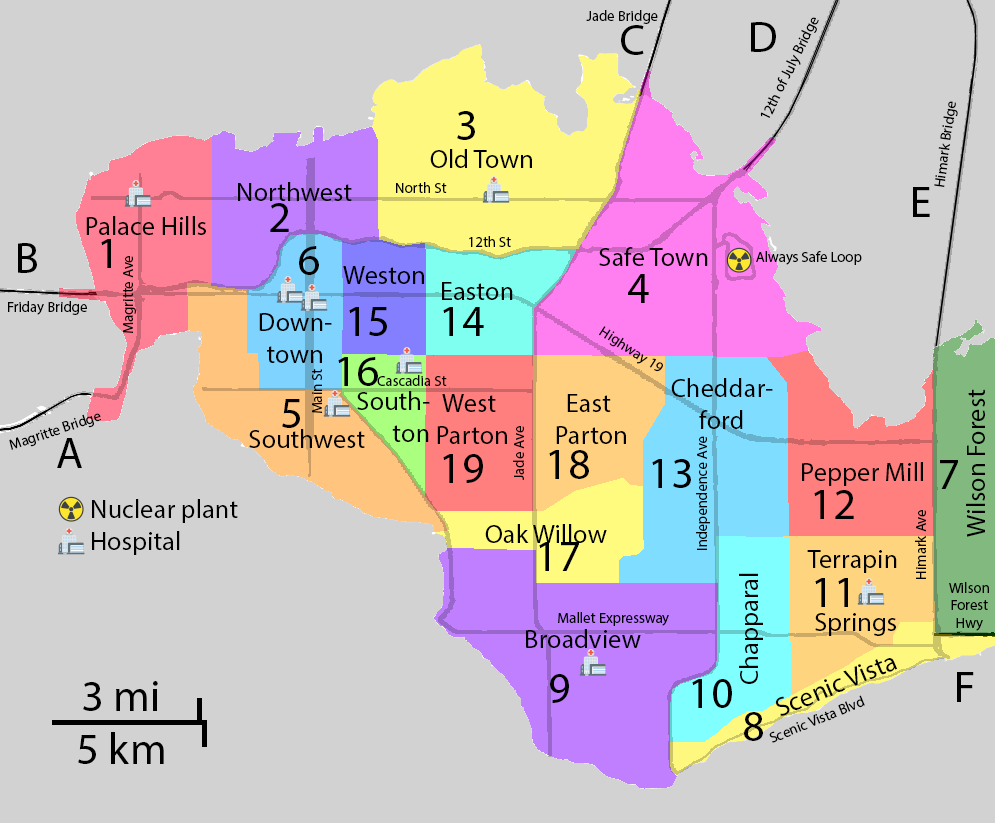
\includegraphics[width=\columnwidth]{Project/figures/StHimarkLabeledMap.png}
    \caption{Map of the city.}
      \label{fig:sthimark}
\end{figure}

\section{Analysis Strategy Outline }

We chose to not plan too strictly ahead of time what our visualizations and filtering steps would be. We compiled a list of possible ways to visualize and filter the data in the beginning of the project, and then we tried out some of them to get acquainted with the data. 

We started with simple graphs of value versus time and used different filters and scaling in order to visualize different aspects of the data. In this step we looked for suspicious sensors and outliers to be able to remove them if necessary. 

Following this we explored the spatial aspects of the data, using choropleths and space time cubes, which allowed us to find interesting areas uncoupled from the sensor ID:s. In the final stage of the project we iterated these three steps in varying order to explore interesting patterns we found along the way. 

We also created density heat maps with the data filtered in different ways in order to detect increased radiation and find areas with too few readings.


\section{Data Characterisation and Preparation}

The dataset for this project contains around 4.2 million rows which is separated in to csv files for mobiles sensors, static sensors and static locations.

Because of the amount of data points we had to preprocess the data and filter out relevant data points for our visualizations. This was made by identifying sensors with highly uncertain readings (see Fig.\ref{fig:Scatterplots} for examples of uncertain sensors), classifying outliers with density-based clustering\cite{Density-basedClustering} and visually estimate the interval of the background radiation for both the mobile sensors and the static sensors.
\begin{figure}[h!]
    \centering
    \includegraphics[scale=0.38]{Project/figures/Scatter1.png}
    \includegraphics[scale=0.38]{Project/figures/Scatter2.png}
    \includegraphics[scale=0.38]{Project/figures/Scatter18.png}
    \includegraphics[scale=0.38]{Project/figures/Scatter26.png}
    \caption{Scatter plots of uncertain mobile sensors}
    \label{fig:Scatterplots}
\end{figure}


Before using density-based clustering we normalized the timestamp and the value of the data points with min-max normalization algorithm\cite{Min-Max}, to be able to specify the minimum euclidean distance between each point and we also set a minimum of four points for a cluster.

The reason for identifying outliers with density-based clustering rather then just classifying the values in to several intervals is that density-based clustering will filter out more of the uncertain data points and still accept fluctuations of the radiation readings which is normal with radiation in both background radiation levels and higher levels of radiation.

Density-based clustering measures the euclidean distance between each data point and group the point in a cluster if conditions of euclidean distance and number of points nearby is meet, so the outliers will be the points that have a high difference in both radiation value and time from the nearby points. (see Fig.\ref{fig:DBScanMobile} & Fig.\ref{fig:DBScanStatic})
\begin{figure}[h!]
    \centering
    \includegraphics[scale=0.15]{Project/figures/Result of DBScan clustering of mobilesensors.png}
    \caption{Density-based clustering of mobile sensors}
    \label{fig:DBScanMobile}
\end{figure}
\begin{figure}[h!]
    \centering
    \includegraphics[scale=0.15]{Project/figures/Result of DBScan cluster for staticsensors.png}
    \caption{Density-based clustering of static sensors.}
    \label{fig:DBScanStatic}
\end{figure}
\newpage
We used Python Pandas dataframes\cite{Pandas} to store the readings in and this made it easy to store several dataframes for all the levels of filtering, to in the end be able make visualisations for different filtering levels. 
For the space-time cubes the data was downsampled to 12 samples per hour using a mean sampling method. 
The data used to animate the points on the Folium map was around 70 000 rows and the heatmaps that was added as layers to the Folium map\cite{Folium} shows the unfiltered data, the filtered data for 60-2500 cpm and filtered data for 150-2500 cpm.  
We decided not to try to align the differences in baselines in the data itself, but only adjusting for it when setting graph parameters such as colorscale. This was since it was not clear what the reason for the different baselines were, which made it difficult to understand how to scale them properly. We could have subtracted the baseline value, but it would also be possible to scale it by multiplying with a normalization factor. Since we did not manage to determine how the bias affected the readings, we chose to not introduce more uncertainty and instead rely on more manual analysis of our different graphs to find small changes and patterns. 

\section{Results}

\subsection{Visualize radiation measurements over time from both static and mobile sensors to identify areas where radiation over background is detected. Characterize changes over time.}

This question was the one we spent the most time and resources exploring in this project. Initially we plotted the value of each sensor over time in simple line graphs, keeping the static sensors and the mobile sensors separate. This allowed us to see some patterns in the data such as a possible contamination. We also plotted the data as scatter plots with the value on the Y-axis and time on the X-axis, where we could see how the spread of the data was and find outliers. We used this to look for sensors that seemed suspicious and investigate them further.

We created choropleths for each day but these did not yield a lot of information due to the different base levels of sensors and big size of the neighborhood areas. From this we learned that we needed higher spatial resolution or some filtering. The only clear pattern seen in these was that there were heightened levels of radiation along the southeast coast (see Figure \ref{fig:choropleths}).

\begin{figure}[h!]
    \centering
    \includegraphics[width=0.49\columnwidth]{Project/figures/april6th.jpg}
    \includegraphics[width=0.5\columnwidth]{Project/figures/april7th.jpg}
    \includegraphics[width=0.49\columnwidth]{Project/figures/april8th.jpg}
    \includegraphics[width=0.49\columnwidth]{Project/figures/april9th.jpg}
    \includegraphics[width=0.49\columnwidth]{Project/figures/april10th.jpg}
    \caption{Choropleths of the average radiation recorded each day for each neighborhood with mobile sensors. Ordered from left to right and then down, note the changing colorscales.}
      \label{fig:choropleths}
\end{figure}

We created space time cubes from the mobile sensor data to get a good overview of the data based on the spatial position of sensors as opposed to the sensor ID. We let color represent the value and capped the color scale to reduce the effect of outliers and differences in baseline between different sensors. We also made space-time cubes simply representing the paths of one or more sensors (as the left image in Figure \ref{fig:contamination}), which allowed us to investigate how groups or individual sensors had moved. This was done to identify possible places of contamination or contaminated vehicles, and look into the movements of sensors which looked suspicious when their data was plotted in line- or scatter plots. As it became clear that the differences in baseline made it difficult to see increases in sensors with lower baseline values, we investigated the line- and scatter plots more carefully to find changes in base line values. We found a number of sensors had a small increase at approximately the same time, and when plotting their paths for this time it became clear that most of them were moving through the same area at that time. This might mean that there was a point of contamination there, but only for a limited time. 
\begin{figure}[h!]
    \centering
    \includegraphics[width=\columnwidth]{Project/figures/mobile_spacetime.png}
    \caption{Space time cube of downsampled data from the mobile sensors. Note that the colorscale has been clamped to the interval 50-100.}
      \label{fig:spacetime_mobile}
\end{figure}
\begin{figure}[h!]
    \centering
    \includegraphics[width=\columnwidth]{Project/figures/static_spacetime.png}
    \caption{Space time cube of downsampled data from the static sensors. Note that the colorscale is on the interval 10-30.}
      \label{fig:spacetime_static}
\end{figure}
\begin{figure}[h!]
    \centering
    \includegraphics[width=0.49\columnwidth]{Project/figures/newplot (9).png}
    \includegraphics[width=0.49\columnwidth]{Project/figures/newplot (10).png}
    \caption{Paths (left) and values (right) of sensors all showing a high increase in radiation at the end of the time interval when investigated through scatterplots. Here it is clear that all but one exit the city by the same route at the same time, meaning this is probably a point of contamination.}
      \label{fig:contamination}
\end{figure}\\

By plotting the higher readings of radiation on a map in Folium we could plot the readings over time and location and also interact with the animation to look closer on certain time periods and locations to verify the information from the space time cubes and identify areas of interest. (See Figure \ref{fig:foliummap}) 

\begin{figure}[h!]
    \centering
    \includegraphics[scale=0.2]{Project/figures/Foliumanimationofreadingsdots.png}
    \caption{Radiation readings from both mobile and static sensors. Where color and size of the dots represent the level of radiation.}
    \label{fig:foliummap}
\end{figure}
\newpage
\subsection{Use visual analytics to represent and analyze uncertainty in the measurement of radiation across the city.}
With the help of heat maps in Folium we could visualize the levels of filtration of the readings on to a map and also overlay the heat maps over each other to see the difference that the filtration does to the uncertainty of the readings over the city.(see Fig.\ref{fig:foliummapheatmapall} & Fig.\ref{fig:foliummapheatmapfiltered})

\begin{figure}[h!]
    \centering
    \includegraphics[scale=0.3]{Project/figures/Heatmapall.png}
    \caption{Heat maps of all radiation readings from mobile and static sensors.}
    \label{fig:foliummapheatmapall}
\end{figure}

\begin{figure}[h!]
    \centering
    \includegraphics[scale=0.3]{Project/figures/Heatmapfiltered.png}
    \caption{Heat maps of the high levels of radiation readings from mobile and static sensors.}
    \label{fig:foliummapheatmapfiltered}
\end{figure}

\subsection{Given the uncertainty you observed in question 2, are the radiation measurements reliable enough to locate areas of concern?}

We believe that when the data is filtered to remove outliers it is possible to find areas of concern that are reliable. One example being the contamination that is clearly present in Figure \ref{fig:contamination}, with values high above the normal range. It is also supported by there being multiple sensors having recorded this increase at the same time. However, the data should be interpreted with caution. For example, the cars that indicate being contaminated all follow the same path, it is possible that not all are contaminated but are recording radiation from just one or a few contaminated vehicles in the group. 

The differences in baseline between the mobile sensors make it difficult to find small increases recorded by the sensors with lower baseline, but analyses of patterns in each sensor's values are of help there. These findings should be cross referenced with the static sensors and other mobile sensors since the mobile sensors seem a bit unreliable at times. The baseline difference also makes it so that visualizations based simply on different types of averages such as the choropleth become dependent on which sensors are in the area. Therefore only large increases should be trusted for these visualization.

\subsection{Summarize the state of radiation measurements at the end of the available period. Use your novel visualizations and analysis approaches to suggest a course of action for the city. Use visual analytics to compare the static sensor network to the mobile sensor network. What are the strengths and weaknesses of each approach? How do they support each other?
}

We suggest that the authorities immediately, close the Wilson Forest Highway and investigate if there is any source of contamination there, due to the results in Figure \ref{fig:contamination}. The owners of those cars should also be contacted and obliged to clean their cars in a specialized facility that can take care of radioactive waste. 

We also propose that Safe Town and the east part of Old town be closed of, and systematically searched for sources of radiation. This is based on the increased radiation levels recorded by both static and mobile sensors.

\subsection{The data for this challenge can be analyzed either as a static collection or as a dynamic stream of data, as it would occur in a real emergency. Describe how you analyzed the data - as a static collection or a stream. How do you think this choice affected your analysis? 
}

We chose to analyze the data as a static collection rather than as a stream of data. This facilitated our iterative approach where we would discover new things about the dataset and investigate them along the course of our analysis. This meant looking at data from before and after the interesting events to determine what kind of event it was, how likely it was to be an error and how important it was. For example, we could see that there were some very high values for a group of sensors towards the end of the time period, which gave us a frame of reference for how high the values could be, that we would not have had if we analyzed the data as a stream.

\section{Design \& implementation of VA solution}

We used Tableau\cite{Tableau} to explore the data and make some initial graphs. This was chosen since it was quite fast for prototyping, but abandoned due to a lack of control for finer features and no support for 3D rendering. 

Most of our visualizations are implemented using Python libraries. We chose this because Python is a well established language with a diverse set of libraries and tools, which suited our approach of trying out new things as we became more familiar with the data. We used the Pandas and Geopandas libraries because we had previous experience using Pandas, and Geopandas seemed to be a well established way of combining data frames with geospatial data. 

To produce the space-time cubes\cite{Spacetime} we used the Plotly and Plotly Express libraries for their speed and simplicity. We also used the Plotly Graph Objects library to construct some space-time cubes with data from two datasets, since this library provided greater control at the cost of some time spent on implementation. 

To produce the animated map and heat maps we used the Folium library in Python because it handles geo coordinates, animation and interaction pretty well both in hindsight it had problems handling all the data points and suffered delays in the animation of the data points. 




\section{Discussion}

We spent a lot of time getting familiar with the data and investigating different findings and hypotheses. In hindsight this led to multiple insights in the end but cost us a lot of time. We think it was necessary to do this familiarization in order to understand the limitations of the data, such as different base levels and lost values, but it could have been more productive if we implemented visualizations such as the space-time cubes earlier. We might also have been more methodical when going through the scatter plots of each sensors value, to detect patterns in an earlier stage. 

The space-time cubes provided a connection of the radiation levels to their spatial position, which was very important for detecting areas with high radiation levels. Their downside was that it was no longer possible to distinguish which sensor each data point came from, which made it necessary to cap the color scale so that it started above the highest baseline measurements. The large amount of data also made them quite cluttered, and it was sometimes difficult to determine the spatial position of a point. It was possible to get the coordinates of a data point by hovering over it with the mouse, but for general analysis this could be time consuming. The space-time cubes were 3D graphs that could be moved and rotated, which also helped the user make sense of the cluttered data. By viewing the data from different angles it was possible to see different aspects of it, and consider different areas. 

To further develop the cubes, it would be useful to allow the user to select which sensors should be displayed. Also what time range and what area, so the user could explore the data with different questions in mind. We implemented graphs of only a selected number of sensors, which was very useful for investigating the spatial behavior of sensors with similar patterns in their values. For these limited datasets it was also useful to create a space-time cube with the paths of each vehicle, but for the full set of mobile sensors that visualization was too cluttered to yield any insight. 

For future work it would be better to implement the animation of data points and heat maps directly in Javascript together with Leaflet\cite{Leaflet} which we think would solve the problem with the animation delays and also opens up to implement more interactive features. 

\section{Conclusions}
We have identified areas of interest and possible contaminated vehicles and suggested a action plan for the city to follow. The problem was solved with dataprocessing and visual analytics where we have justified our choices and clarified how we handled the uncertainties of the readings. 



\bibliographystyle{abbrv}

%%use following if all content of bibtex file should be shown

\bibliography{refs}

\section*{Contributions from Each Project Member}\label{cont}

\begin{description}
\item[Author Alexander Lindell] {
Written on all parts of the report and mainly work on the data preparation with filtering and density-based clustering , plotting scatter plots, heat maps in Folium and animation in folium.}
\item[Author Emilia Ståhlbom] {
Written on all parts of the report and mainly work on the data preparation with filtering , choropleths maps and space time cubes.}


\end{description}


\end{document}
